\section{Methodology}
This work is an extension of a wonderful paper \textit{`Applying Occam's Razor
to Transformer-Based Dependency Parsing: What works, What doesn't, and What is
really necessary'}\cite{steps-parser}. The parser is named STEPS(Stuttgart
Transformer based Extensible Parsing System) which indeed is a very flexible
parsing system. The idea is to use a multilingual parser which is trained on
multilingual BERT embeddings. Most of the work here follows the future
directions directed by the authors\cite{steps-parser} while combining some
concepts from UDapter\cite{udapter}. Finally, after all the experiments and
source language/size analysis, we parse Nepali sentences as a zero-shot case.

\begin{figure}[!h]
    \center
    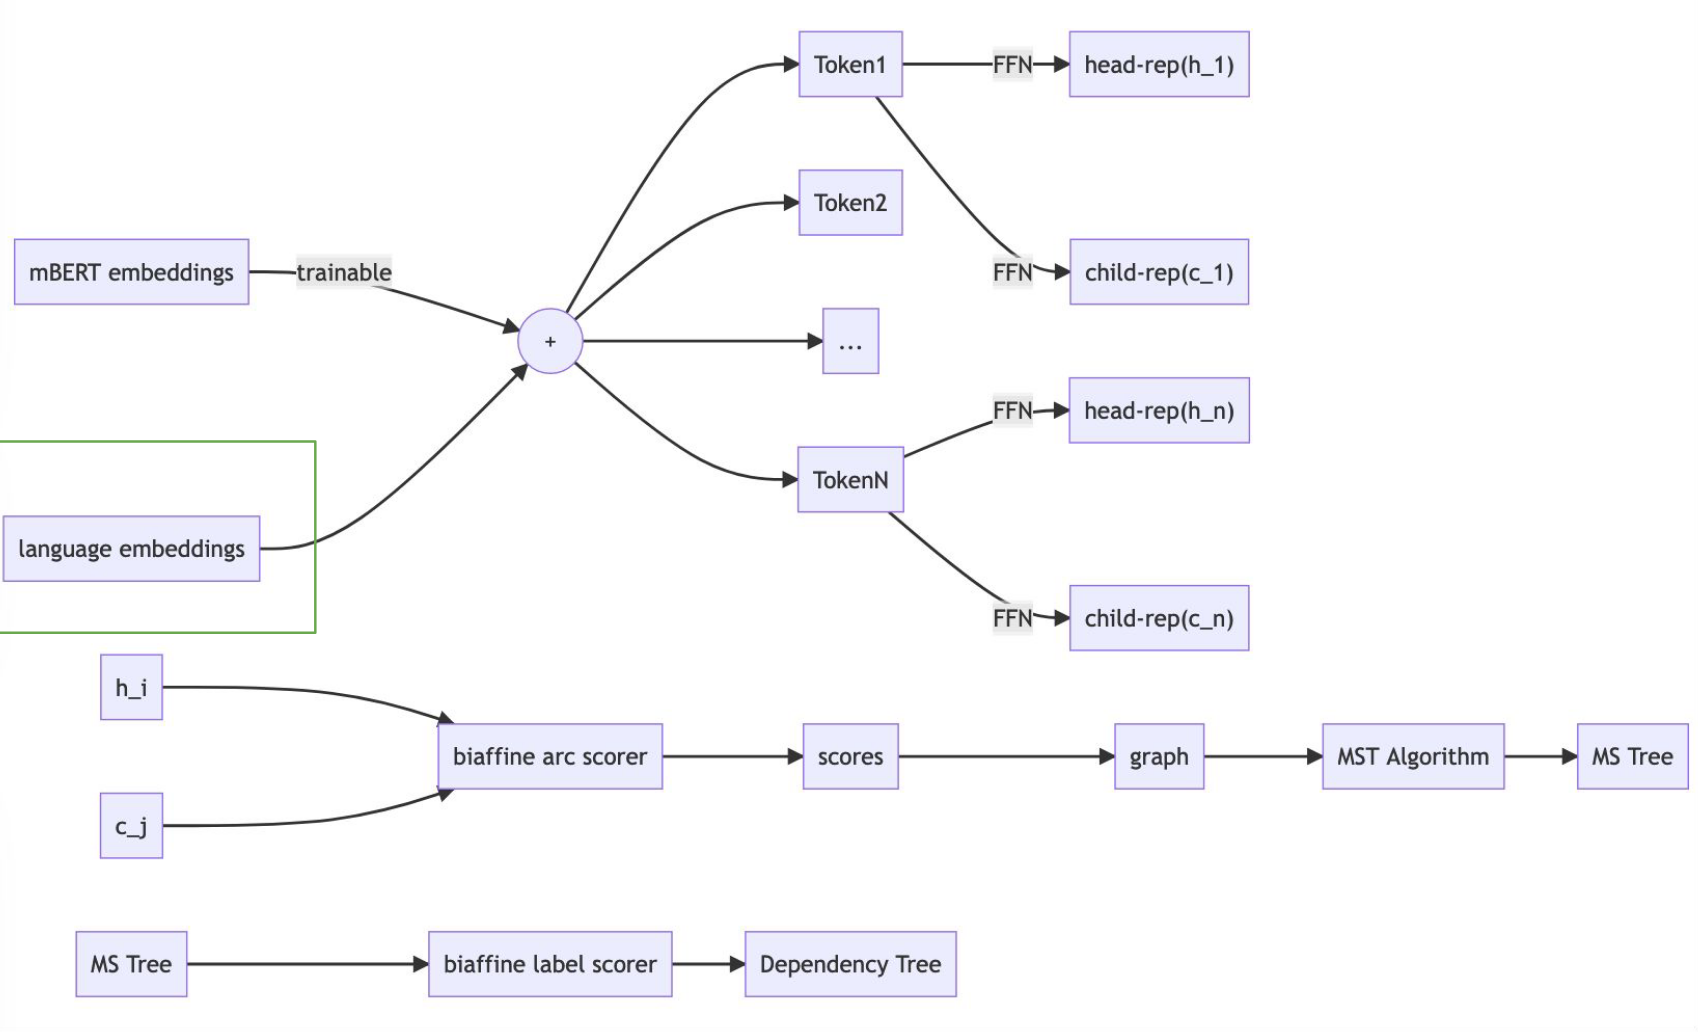
\includegraphics[scale=0.15]{images/Thesis_Architecture}
    \caption{System Architecture}
    \label{system_architecture}
\end{figure}

\section{Neural Graph-based Dependency Parsing}
This is the core idea behind the parser. We use neural graph-based parsing which works as follows:
\begin{itemize}
    \item[1.] For each word $w_i$, find scores for other words $w_j$ as the head of $w_i$ using some scoring function $S$ which will be a Biaffine classifier.
    \item[2.] This will give a set of edges which form a graph.
    \item[3.] Apply Maximum Spanning Tree Algorithm (CLE algorithm) to find the dependency arcs.
    \item[4.] For each arc, find the best scoring arc label, again using some scorer which will be a Biaffine classifier as well.
\end{itemize}

\section{System Architecture}
The latest advances in dependency parsing make use of contextualized language
embeddings like BERT, elmo and XLM-R. This work is an implementation of graph
based dependency parsing using pretrained BERT embeddings which are fine-tuned
as the model gets trained. The architecture is shown in figure
\ref{system_architecture} and the components are described below:

\subsection{mBERT Token Representations}
BERT is a contextualized Masked Language Model(MLM) that has proven to be very
effective for downstream tasks including dependency parsing. Since we are
aiming for transfer learning across various languages, monolingual BERT
embeddings are not adequete. Fortunately, multilingual BERT embeddings are
found for 104 languages, one of whom is Nepali. XLM-R have also shown to
provide better results but Nepali Embeddings are not available.  This makes
token representation using mBERT a natural choice for our task at hand.
The embeddings are fine tuned as the model is trained for dependency parsing.

\subsection{Language Embeddings}
Language embeddings are added at the later parts of the experiment. Since
different languages have different syntactic structures, training a
multilingual parser is a bit tricky. In our case, although Nepali and Hindi
have similar syntactic structures, English is quite different. And this results
in dependency annotations in Nepali or Hindi contradict to that in
English. Similar to \cite{udapter}, we use language embeddings from URIEL and
WALS databases provided by a library called \textit{lang2vec} which itself is
based on \cite{lang2vec}. However, we differ in that, while \cite{udapter} use
all of the 289 sparse features and train a linear model as a contextual
parameter generator, we reduce the dimensions to 18 to make them dense and
directly concat with the mBERT embeddings.

\subsection{Head and dependent representations}
The token representations(mBERT embeddings) obtained are passed to two
different Feed Forward Networks(FFNs) to get their representations as head and
as a child(dependent). Let $r_i$ be embedding vector for each token then,
$$h_i^{head} = FFN^{head}(r_i)$$
$$h_i^{dep} = FFN^{dep}(r_i)$$
Each of the input tokens will have two representations, one for head and another for child.

\subsection{Biaffine Classifier}
This is a scoring function defined as,
$$s_{i,j} = Biaff(h_i^{head}, h_j^{dep})$$
$$Biaff(x, y) = x^\top \textbf{U}y + \textbf{W}(x \oplus y) + \textbf{b}$$
where $\textbf{U}$, $\textbf{W}$ and $\textbf{b}$ are learned parameters and
$\oplus$ represents vector concatenation.

\subsection{Arc and label scoring}
This work uses \textbf{factorized} method for arc and label scoring in which,
arcs are scored first and based on the result, labels are scored. This can also
be done using \textbf{unfactorized} method but this gives no better result and
has more parameters.
\\~\\
Arc Scorer is a biaffine function which takes in every combination of
head-child tokens and assigns scores for each. Then a standard Maximum Spanning
Tree algorithm(generally CLE) is used to find relevant arcs.
\\~\\
Label scorer is also a biaffine function which takes in the arcs of the parsed
spanning tree and assigns corresponding labels.

\section{Evaluation and Validation}
\subsection{Evaluation Metrics}
The two widely used evaluation metrics for dependency parsing are:
\begin{itemize}
    \item \textbf{LAS}: Labeled Attachment Score is the percentage of correct head-modifier labeling among the expected relations.
    \item \textbf{UAS}: Unlabeled Attachment is the percentage of correct head-modifier relations identified among the expected relations.
\end{itemize}
As an example, consider the following ground truth of dependency relations
\begin{verbatim}
Index  Token      Head  Label
-----  -----      ----  -----
1      Book       0     root
2      me         1     dobj
3      a          4     det
4      flight     1     nobj
5      to         6     prep
6      Kathmandu  4     nmod
7      .          1     punct
\end{verbatim}
If the predicted relations are:
\\~\\
\begin{verbatim}
Index  Token      Head  Label  Head-correct?  Label-correct?
-----  -----      ----  -----  -------------  --------------
1      Book       0     root   yes            yes
2      me         1     dobj   yes            yes
3      a          4     amod*  yes            no
4      flight     1     nobj   yes            yes
5      to         5*    prep   no             yes
6      Kathmandu  4     aux*   yes            no
7      .          3*    punct  no             yes
\end{verbatim}
The LAS score is $\frac{correct-head-label-predictions}{total-relations} = \frac{3}{7} = 0.43$\\
The UAS score is $\frac{correct-head-predictions}{total-relations} = \frac{5}{7} = 0.71$

\section{Datasets}
Ideally, we would have a dataset from Universal Dependencies treebank.
Unfortunately, no such dataset exists as of now and thus 200 validation
sentences for Nepali had to be generated manually. Dataset of similar size has
been used by Lim et al(2018)\cite{multilingualCaseStudy} and in other zero shot
and low resource settings\cite{udapter}\cite{zero-shot} which led us to assume
that 200 should be a good enough validation size. A glimpse of what UD Treebank
dataset looks like is shown in Figure \ref{ud_structure}. The gold labels
defined in UD are show in Appendix \ref{ud_labels}.

\subsection{Training Datasets}
UD Treebank consists of rich collection of dependency parsing
annotations for various languages. Unfortunately, Nepali dependency
annotated datasets are not available in the treebank. Since this is a
transfer learning setup, we choose a subset of languages data in the treebank.
The languages are tabulated below in table \ref{table:dataset_summary}.
\begin{table}[!ht]
    \begin{center}
        \begin{tabular}{|l|l|c|}
            \hline
            \textbf{Language} & \textbf{Code} & \textbf{Dataset size} \\
            \hline
            Arabic & ar & 1500 \\
            \hline
            English & en & 1500 \\
            \hline
            Basque & eu & 1500 \\
            \hline
            Finnish & fi & 1500 \\
            \hline
            Hebrew & he & 1500 \\
            \hline
            Hindi & hi & 1500 \\
            \hline
            Italian & it & 1500 \\
            \hline
            Japanese & ja & 1500 \\
            \hline
            Korean & ko & 1500 \\
            \hline
            Russian & ru & 1500 \\
            \hline
            Swedish & sv & 1500 \\
            \hline
            Turkish & tr & 1500 \\
            \hline
            Chinese & zh & 1500 \\
            \hline
        \end{tabular}
        \caption{Dataset languages}
        \label{table:dataset_languages}
    \end{center}
\end{table}
These 13 languages were chosen as suggested in \cite{udapter}. The
languages consist of almost all the families of languages spoken in the world
so that the transfer learning becomes efficient.

\begin{figure}[!ht]
    \center
    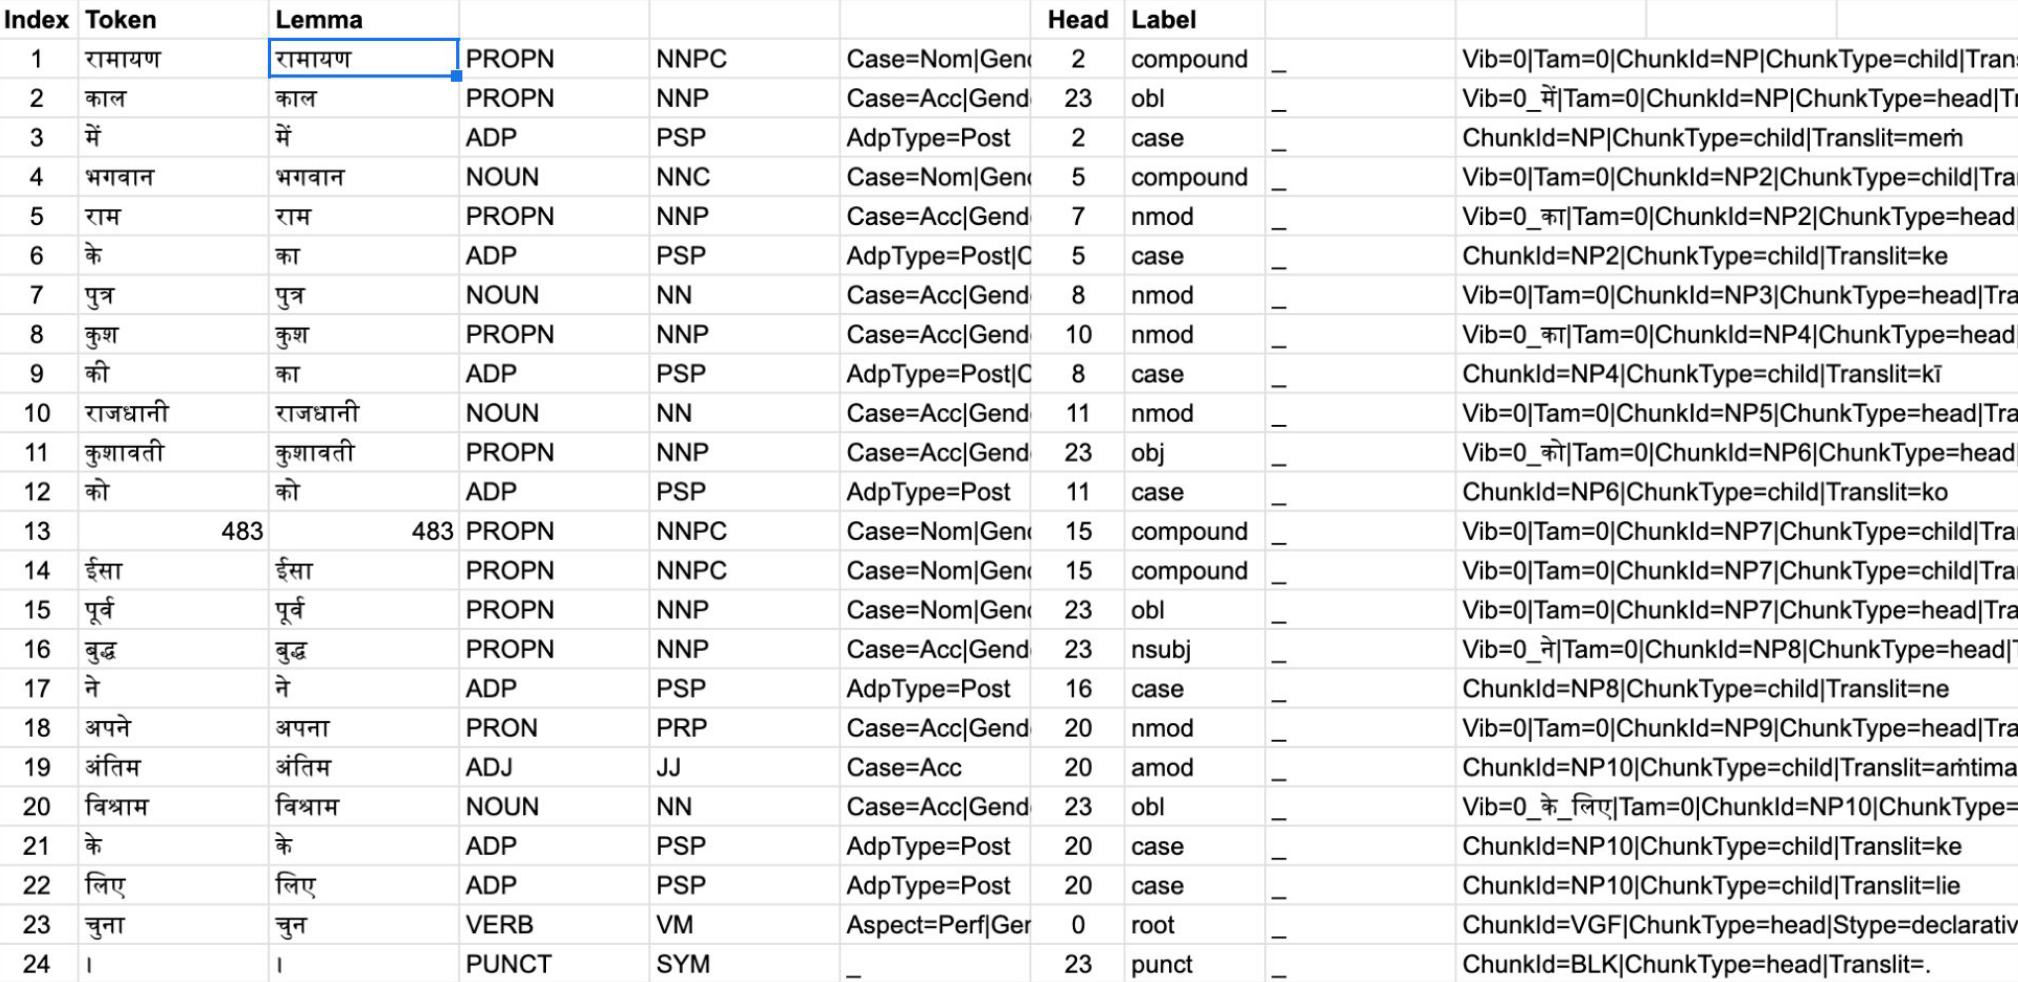
\includegraphics[scale=0.16]{images/ud_structure}
    \caption{Sample data in UD Treebank}
    \label{ud_structure}
\end{figure}

The dependency tree of an annotated sentence is shown in Figure \ref{dep_tree_example}
\begin{figure}[!ht]
    \center
    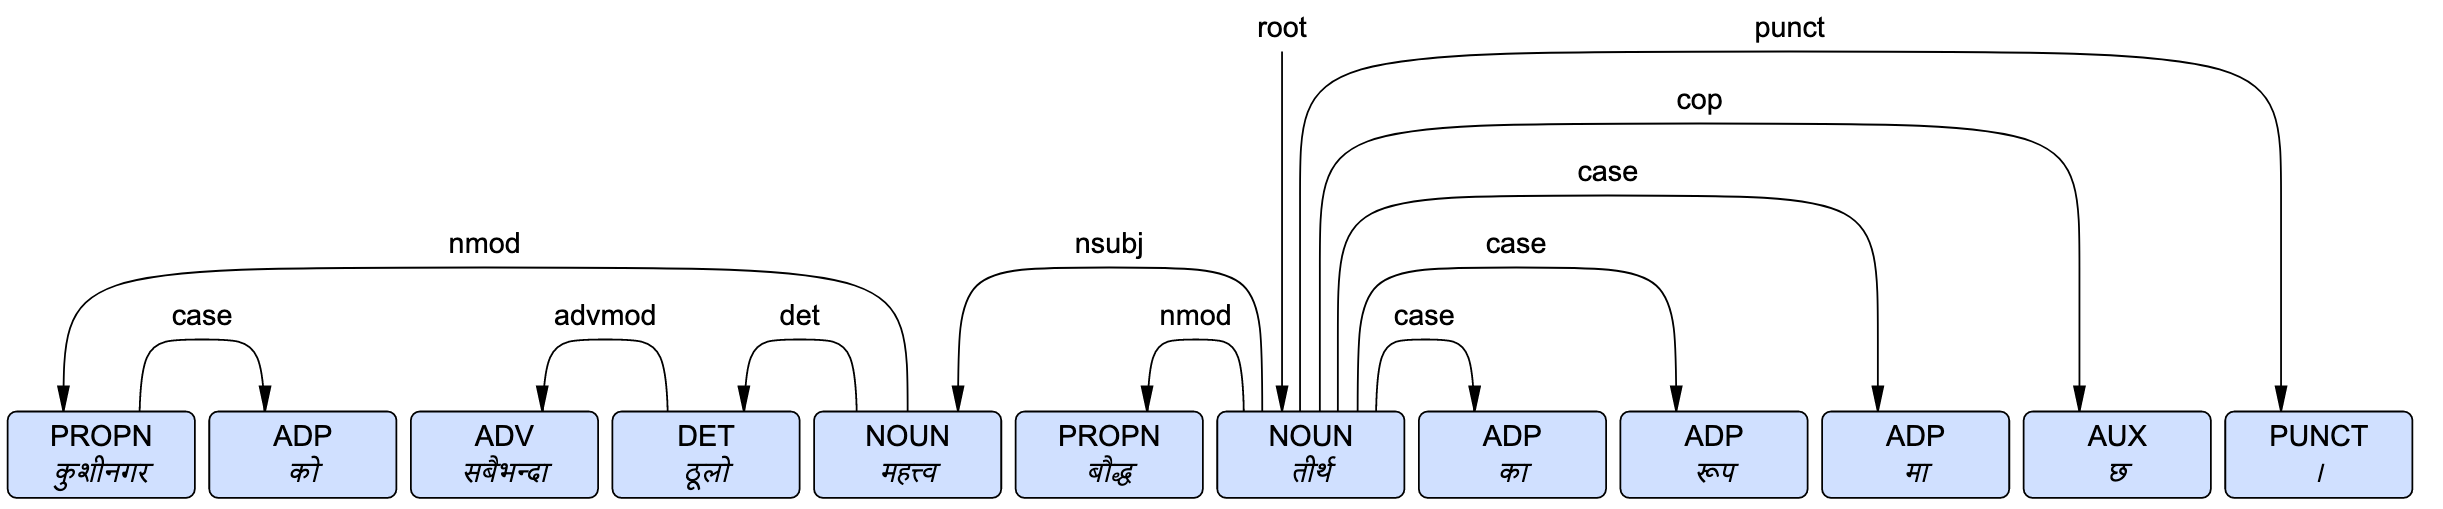
\includegraphics[scale=0.15]{images/nepali_dependency_parse}
    \caption{Dependency tree for a sentence in dataset}
    \label{dep_tree_example}
\end{figure}

\subsection{Validation Dataset}
As can be seen from Figure \ref{ud_structure} that manually creating dataset is
a long and tedious process even though only the columns \textit{Index, Token,
Head and Label} are required for dependency parsing. It is interesting to see
that since Hindi and Nepali language are very similar, if we have token-wise
translations of Hindi data, every other column can be reused except for the
\textit{Lemma} column. This work adopts the translation and alignment of Hindi
sentences in order to create an equivalent Nepali dataset. The following steps
were carried out while creating validation dataset:
\begin{itemize}
    \item[1.] Certain portion of the test dataset for Hindi was taken from the UD treebank. It is possible to align Hindi and Nepali while it's very hard for languages like English.
    \item[2.] It was preprocessed to obtain raw sentences. Each token was carefully preserved.
    \item[3.] The sentences were bulk translated by Google Translation and tokenized.
    \item[4.] However, the translations were not aligned. So a simple interactive tool was created that allowed manual corrections of wrong alignments.
    \item[5.] The results were verified by a fluent Hindi-Nepali speaker, whose summary is presented in Appendix \ref{translation}.
\end{itemize}
A summary of the dataset is shown below in Table \ref{table:dataset_summary}.
Incorrect translation summary is presented below in Table \ref{table:incorrect_summary}. Full enumeration of incorrect
translations is present in Appendix \ref{translation}.

\begin{table}[ht]
    \begin{center}
        \begin{tabular}{|l|c|}
            \hline
            Dataset Domain & Hindi News \\
            \hline
            Total Sentences & 200 \\
            \hline
            Total tokens & 3360 \\
            \hline
            Maximum tokens per sentence & 44 \\
            \hline
            Minimum tokens per sentence & 3 \\
            \hline
            Average tokens per sentence & 13 \\
            \hline
        \end{tabular}
        \caption{Dataset summary}
        \label{table:dataset_summary}
    \end{center}
\end{table}

\begin{table}
    \begin{center}
        \begin{tabular}{|l|c|}
            \hline
            Total Tokens & 3360 \\
            \hline
            Sentences with one or more errors & 31 \\
            \hline
            Incorrect token translations & 40 \\
            \hline
            Incorrect translation percentage & 1.19\% \\
            \hline
        \end{tabular}
        \caption{Incorrect translation summary}
        \label{table:incorrect_summary}
    \end{center}
\end{table}

\begin{figure}[!h]
    \center
    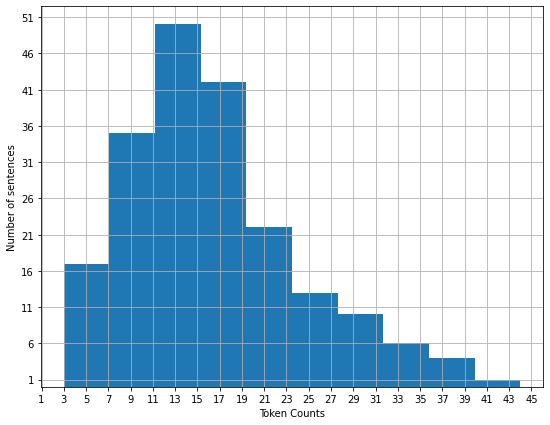
\includegraphics[scale=0.3]{images/dataset_histogram}
    \caption{Sentences - tokens count histogram}
    \label{tokens_count_histogram}
\end{figure}
Sample sentences are shown in Appendix \ref{dataset_summary_sample_appendix}.
\newpage

At first glance it might seem that having a 200 sentence tagged dataset might
not be sufficient even for validation/testing, let alone for training. However,
as we can see on the following table(parts copied from \cite{udapter}), on
average of only about 150 sentences are used for testing purposes.

\begin{table}[ht]
    \begin{center}
        \begin{tabular}{|c|c||c|}
            \hline
            \textbf{Language} & \textbf{Language Code} & \textbf{Dataset size} \\
            \hline
            Marathi & mr & 47 \\
            \hline
            Sanskrit & sa & 230 \\
            \hline
            Tamil & ta & 120 \\
            \hline
            Telugu & te & 146 \\
            \hline
            Bhojpuri & bho & 254 \\
            \hline
            \textbf{Average} & - & 159 \\
            \hline
        \end{tabular}
        \caption{Zero shot target dataset sizes}
        \label{table:zero_shot_dataset_sizes}
    \end{center}
\end{table}


\section{Results and Analysis}
\section{Experiments and Results}
All the datasets are used from UD treebank and the base implementation is by
\cite{steps-parser} which has been modified to include language embeddings as
well. We carry out series of experiments varying the languages, data sizes and language embeddings.
The following is the tabulation of experiments conducted and the results:
\begin{table}[ht]
    \begin{center}
        \begin{tabular}{|c|c|c|c|c|c|}
            \hline
            \textbf{Exp. code} & \textbf{Languages} & \textbf{Dataset Size} & \textbf{Embeddings?} & \textbf{UAS} & \textbf{LAS} \\
            \hline
            rand & - & 0 & No & 12.75 & 3.48 \\
            \hline
            en2k & en & 2000 & No & 37.47 & 22.41 \\
            \hline
            en5k & en & 5000 & No & 38.30 & 22.68 \\
            \hline
            en & en & 10000 & No & 39.17 & 23.9 \\
            \hline
            hi & hi & 13000 & No & 50.74 & 39.32 \\
            \hline
            en\_hi & en,hi & 15000 & No & 41.31 & 32.67 \\
            \hline
            multi & multi & 18000 & No & 59.52 & 47.47 \\
            \hline
            multi\_np20 & \textbf{np},multi & 18020 & No & 71.22 & 59.97 \\
            \hline
            \textbf{multi\_np100} & \textbf{np},multi & 18100 & No & \textbf{76.98} & \textbf{67.29} \\
            \hline
            hi\_np20 & \textbf{np}, hi & 13020 & No & 69.59 & 60.79 \\
            \hline
            \textbf{hi\_np100} & \textbf{np},hi & 13100 & No & \textbf{80.73} & \textbf{72.67} \\
            \hline
            \textbf{np100} & \textbf{np} & 100 & No & \textbf{49.86} & \textbf{36.84} \\
            \hline
            \hline
            en2kem & en & 2000 & Yes & 32.43 & 23.07 \\
            \hline
            en5kem & en & 5000 & Yes & 32.66 & 22.31 \\
            \hline
            enem & en & 10000 & Yes & 35.79 & 24.2 \\
            \hline
            hiem & hi & 13000 & Yes & 52.18 & 40.71 \\
            \hline
            en\_hi\_em & en, hi & 15000 & Yes & 44.16 & 33.15 \\
            \hline
            multiem & multi & 18000 & Yes & 59.05 & 47.19 \\
            \hline
            \textbf{multi\_np20em} & \textbf{np},multi & 18020 & Yes & \textbf{71.22} & \textbf{59.43} \\
            \hline
        \end{tabular}
        \caption{Experiments and results}
        \label{table:experiments_results}
    \end{center}
\end{table}
The \textbf{multi} languages are the languages mentioned in Table \ref{table:dataset_languages}.

\begin{figure}[!h]
    \center
    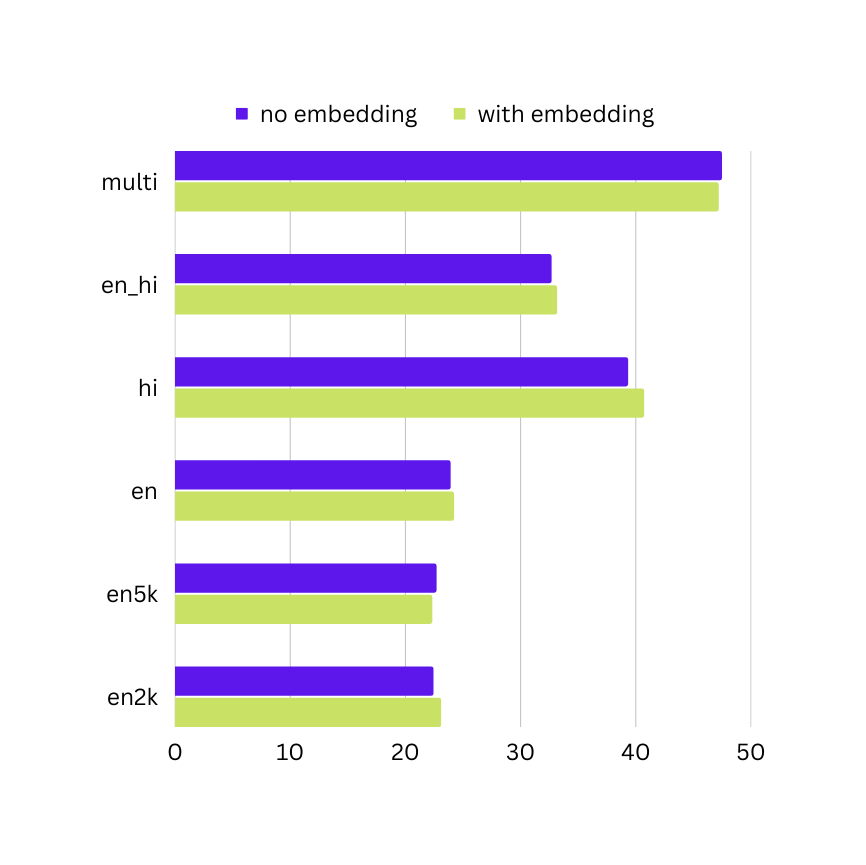
\includegraphics[scale=0.3]{images/results}
    \caption{Effects of language embeddings for zero-shot case}
    \label{results}
\end{figure}

\begin{figure}[!h]
    \center
    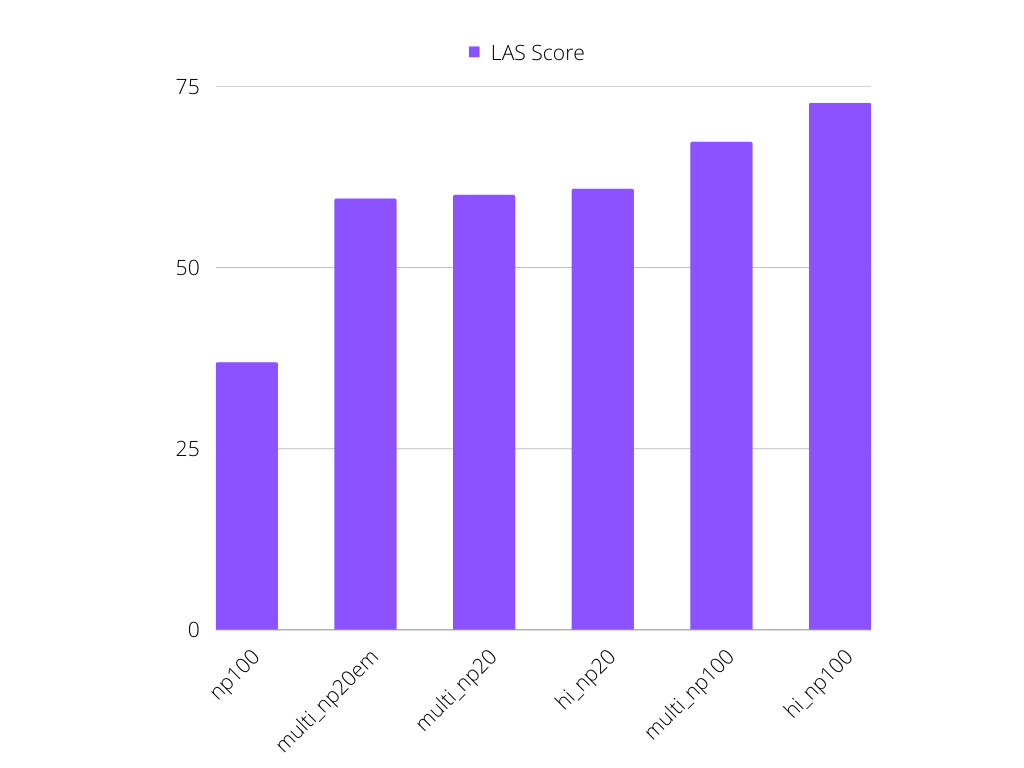
\includegraphics[scale=0.3]{images/fewshot_comparison}
    \caption{Comparison of fewshot experiments}
    \label{fewshot_comparison}
\end{figure}


The results are also summarized in Figure \ref{results}. So far, the best zero
shot LAS obtained is 47.38 for multi-source setup. We consider the previous
results on indic languages like Bhojpuri, Marathi, Sanskrit as the baseline.
Combining the results of \cite{zero-shot}\cite{udapter} for zero shot indic
languages like the highest average LAS obtained is \textbf{44.1}. Our result is
slightly better than the average. For the \textbf{few-shot} case where we used 20
Nepali sentences for training along with other languages, we have the highest
LAS score of \textbf{61.34} whereas with 100 Nepali sentences with
other languages, the score is 76.98. The result of parse on a sample sentence is shown in Figure \ref{img:sample_result1}

\section{Analysis}
The upper portion of table \ref{table:experiments_results} shows the results
when the original architecture by \cite{steps-parser} is used. The lower
portion shows the corresponding results when language embeddings is
incorporated in the architecture except for the random initialization. The
experiment codes are just for the shorthand names in graph.
\\~\\
Looking at the individual sections it is clear that some data is better than no
data and English as source underperforms Hindi as source. This is just a
verification of our intuition and underlying typographical relations of English
and Hindi with Nepali. Combining Hindi and English slightly degrades
performance in both sections which is also expected.
\\~\\
\textbf{Explanation of multi}\\
For multi language sources, we used the setup used by UDapter\cite{udapter}.
They use 13 different language-typologically diverse languages from over the
world. And it shows that the performance does increase significantly. Dataset
size has been made equal(around 12000 sentences) for each experiments that do
not explicitly mention size.
\\~\\
\textbf{Few-shot learning}\\
On the last rows of each section, the experiment names suffixed by
\textit{\_np*}, we present the results of few-shot learning where we used some
Nepali tagged sentences for training. As anyone would have anticipated, this
has increased the accuracy. It was not expected, however, that the difference
would be as big as 17\% even for just 20 Nepali sentences for training. And for
100 Nepali sentences in source training, the LAS scores obtained are 72.67\%.
This suggests that significant improvements in the scores can be obtained when
more Nepali sentences are used
as training.
\\~\\
\textbf{Effect of language embeddings}\\
Including language embeddings in the original architecture definitely shows
some improvements. The improvements are, however, not very significant. For the
case of multiple languages, the performance even decreases slightly. This might
be experimental error but we still have to investigate on this.
\\
The effect of concatenated language embeddings also seemed to be slightly
detrimental for few-shot cases. This perhaps indicates that for multi-source
training, mBERT already contains enough information about the languages
typology and concatenating language embeddings causes the effect of increased
training parameters to outweigh the increased accuracy due to language embeddings.
\\~\\
\textbf{Fully supervised learning}\\
We also evaluated the model when it was fully supervised by Nepali sentences
only.  For this, we split the 200 sentences as 100, 20 and 80 for training,
validation and testing respectively. The LAS score obtained is 36.84 which is
tabulated on the last row of upper experiments table. The score is clearly
better than using just English sentences for training. This is due to Nepali
language's dissimilarity with English. However the score is  slightly less than
training using Hindi only. This is because Nepali and Hindi are similar and
that the size of Hindi corpus is much bigger(~13k sentences) compared to
Nepali(100 sentences).
\\~\\
\textbf{Effect of Source Langauges}\\
For zero shot case, we can see from above table that using the 13
languages(multi) shows better score than when using Hindi only or Hindi and
English only. However for few-shot scenario, we can see that multi setup has
slightly less score than when using Hindi only(59.97 vs 60.79 for 20 sentences
and 67.29 vs 72.67 for 100 sentences). This suggests that when the target
language(Nepali) sentences are present in training, including typologically
dissimilar languages for training result in some level of noise for the parser.

\subsection*{Resources Used}
Majority of the experiments were run on AWS g4dn EC2 instance which has NVIDIA
T4 GPU.  Each experiment on average required around 13 hours. Some preliminary
runs were done on a workstation in LICT. The computation times for each
experiments are tabulated in Appendix \ref{experiments_time_appendix}.

\begin{figure}[!h]
    \center
    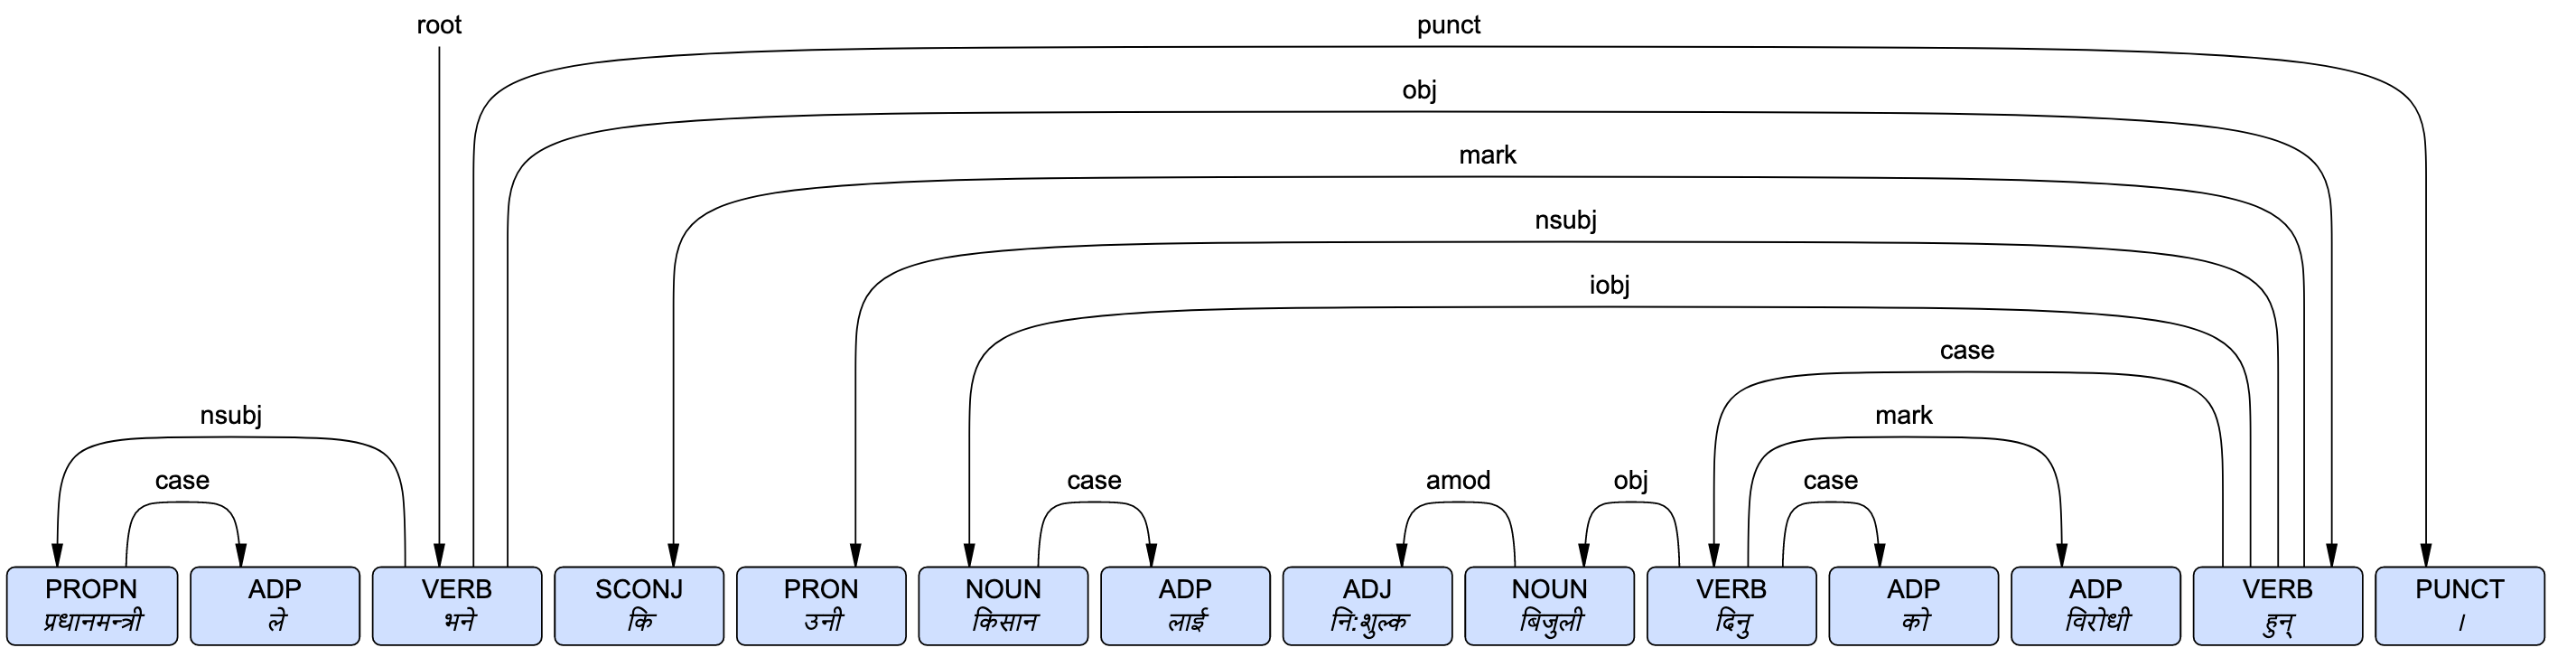
\includegraphics[scale=0.18]{images/sample_result}
    \caption{Sample parse of \dev{प्रधानमन्त्री ले भने कि उनी किसान लाई नि:शुल्क बिजुली दिनु को विरोधी हुन् ।}}
    \label{img:sample_result1}
\end{figure}
\section{Conclusions and Future Work}
The most important part of any machine learning system is the dataset.
In the case of Nepali dependency parsing, there have been no annotated
dataset. Manual annotation is a time consuming and technical task
especially in the case of Nepali dependency tags. In this work, the
task has been made easier by translating some parts of existing Hindi
treebank data and semi-automatically aligning the original Hindi and
translated Nepali sentences. Since Hindi and Nepali are similar, this
alignment allows to reuse the annotations for Hindi and saves a lot of
time. The dataset is also validated by a fluent Hindi-Nepali speaker.

After preparing the dataset, an existing state-of-the art Neural
Graph Parser was customized for transfer learning and a dependency
parser for Nepali was created and analyzed. A good baseline LAS score
of 72 has been achieved.

There are still spaces for improvement of the system. This work can be
extended in future to achieve the following:
\begin{itemize}
    \item [1.] Create more annotations.
    \item [2.] Experiment with source language variations.
    \item [3.] Fine tune BERT with language specific features.
\end{itemize}
